\documentclass[border=1cm]{standalone}
\usepackage{tikz}
\usetikzlibrary{calc}

\begin{document}

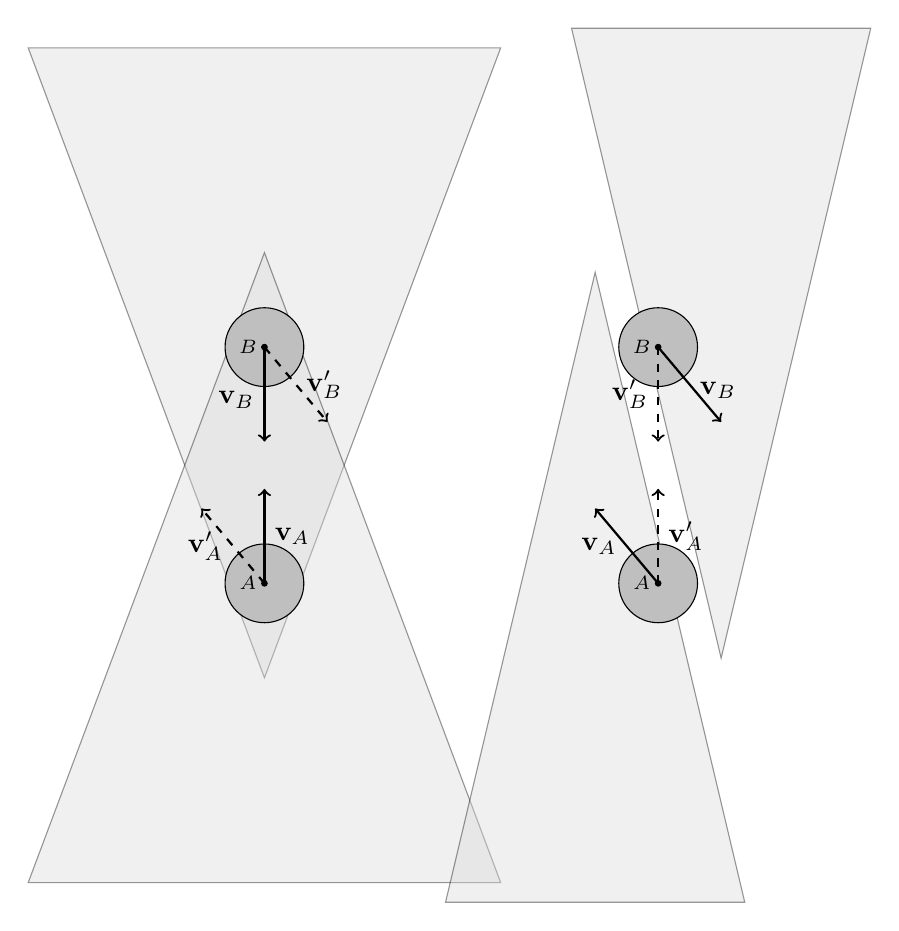
\begin{tikzpicture}
% [trim left=1cm, trim right=1cm, trim top=1cm, trim bottom=1cm]
    % Define points for A and B
    \coordinate (pA) at (0,0);
    \coordinate (pB) at (0,3);

    \coordinate (v) at (0,-1.2);

    % Draw shaded velocity obstacle cone with black outline
    \filldraw[gray!30, draw=black, thin, opacity=0.4] ($(pA) + (v)$) -- ++(-3, 8) -- ++(6,0) -- cycle;
    \filldraw[gray!30, draw=black, thin, opacity=0.4] ($(pB) - (v)$) -- ++(-3, -8) -- ++(6,0) -- cycle;
    
    % Draw shaded circles with black outline
    \filldraw[gray!50, draw=black, thin] (pA) circle (0.5cm);
    \filldraw[gray!50, draw=black, thin] (pB) circle (0.5cm);

        % Draw points at the centers of the circles
    \filldraw[black] (pA) circle (1pt);
    \filldraw[black] (pB) circle (1pt);


    % Label points, offset down and to the left
    \node at ($(pA) + (-0.2,0)$) {$_A$};
    \node at ($(pB) + (-0.2,0)$) {$_B$};

    % Draw vector arrows and label velocity above the middle of the vector
    \draw[->, thick] (pB) -- ++(v) node[midway, left, yshift=-02] {$\mathbf{v}_B$};
    \draw[->, thick] (pA) -- ++($(0,0) - (v)$) node[midway, right, xshift=0pt] {$\mathbf{v}_A$};

    \draw[->, thick, dashed] (pA) -- ++(-0.8, 0.95) node[midway, left] {$\mathbf{v}_A^{\prime}$};
    \draw[->, thick, dashed] (pB) -- ++(0.8, -0.95) node[midway, right] {$\mathbf{v}_B^{\prime}$};


% NEXT STATE
    % Define points for A and B
    \coordinate (pAp) at (5,0);
    \coordinate (pBp) at (5,3);

    \coordinate (vp) at (0.8, -0.95);

    % Draw shaded velocity obstacle cone with black outline
    \filldraw[gray!30, draw=black, thin, opacity=0.4] ($(pAp) + (vp)$) -- ++(-1.9, 8) -- ++(3.8,0) -- cycle;
    \filldraw[gray!30, draw=black, thin, opacity=0.4] ($(pBp) - (vp)$) -- ++(-1.9, -8) -- ++(3.8,0) -- cycle;
    
    % Draw shaded circles with black outline
    \filldraw[gray!50, draw=black, thin] (pAp) circle (0.5cm);
    \filldraw[gray!50, draw=black, thin] (pBp) circle (0.5cm);

        % Draw points at the centers of the circles
    \filldraw[black] (pAp) circle (1pt);
    \filldraw[black] (pBp) circle (1pt);

    % Label points, offset down and to the left
    \node at ($(pAp) + (-0.2,0)$) {$_A$};
    \node at ($(pBp) + (-0.2,0)$) {$_B$};

    % Draw vector arrows and label velocity above the middle of the vector
    \draw[->, thick] (pBp) -- ++(vp) node[midway, right, yshift=-02] {$\mathbf{v}_B$};
    \draw[->, thick] (pAp) -- ++($(0,0) - (vp)$) node[midway, left, xshift=0pt] {$\mathbf{v}_A$};

    \draw[->, thick, dashed] (pAp) -- ++($(0,0) - (v)$) node[midway, right] {$\mathbf{v}_A^{\prime}$};
    \draw[->, thick, dashed] (pBp) -- ++(v) node[midway, left] {$\mathbf{v}_B^{\prime}$};


\end{tikzpicture}

\end{document}
